\documentclass[UTF8,a4paper,11pt]{book}
\usepackage[scheme=plain]{ctex}
\linespread{1.1}

%\usepackage{fontspec}
%\setCJKmainfont{FZNewShuSong-Z10}
%\usepackage{lmodern}
\usepackage{amssymb,amsmath,amsthm}
\usepackage{physics}
\usepackage{graphicx}
\usepackage{geometry}
\usepackage{hyperref}
  \hypersetup{
            colorlinks
            }
\usepackage{siunitx}
  \sisetup{range-phrase = --}

\usepackage[dvipsnames]{xcolor}
\usepackage[many]{tcolorbox}

\newtheoremstyle{mystyle}%
  {}%
  {}%
  {}%
  {}%
  {\sffamily\bfseries}%
  {.}%
  { }%
  {}%

\theoremstyle{mystyle}{
  \newtheorem{example}{Example}
}

\tcolorboxenvironment{example}{
boxrule=0pt,
boxsep=0pt,
colback={White!90!Cerulean},
enhanced jigsaw,
borderline west={2pt}{0pt}{Cerulean},
sharp corners,
before skip=10pt,
after skip=10pt,
breakable,
}


% set default figure placement to htbp
\makeatletter
\def\fps@figure{htbp}
\makeatother

%\begin{itemize}
%\item 
%\item 
%\item 
%\item 
%\item 
%\end{itemize}




\date{}

\begin{document}

\tableofcontents

\chapter{Introduction}
Imaging technology enables seeing inside the
body non-invasively[非切入].
Applications of imaging in medicine:
 \begin{itemize}
 \item Diagnostic imaging (aka. what's wrong?)
 \item Therapy planning (aka. how to treat?)
 \item Surgical guidance (aka. treating properly?)
 \end{itemize}

Imaging is an integral [必需] part of modern
medicine.
Used in almost all medical disciplines,
especially:
\begin{itemize}
\item Radiology [放射科]
\item Surgery
\item Oncology [肿瘤科]
\item Neurology
\item Cardiology [心脏病]
\item Urology [泌尿科学]
\end{itemize}

Many types of imaging technology, each with
own strengths and limitations.
\begin{itemize}
\item X-ray imaging 
\item Computed tomography\footnote{X-ray, Ultrasonic} (CT) [计算机断层成像]
\item Ultrasound
\item Magnetic Resonance Imaging (MRI)
\item Positron Emission Tomography (PET) [正电子发射计算机断层扫描]
\end{itemize}
 Different operating principles.
 Choice of imaging method(s) depends on
application.

%\hypertarget{lecture-1}{%
%\subsection{Lecture 1}\label{lecture-1}}
\section{X-ray imaging}


\chapter{Radiation physics related to imaging}
The radiation \textbf{source} produces the radiation
(typically x-rays or gamma rays).
 The radiation \textbf{beam} travels from the source to
the matter.
 The \textbf{matter} is different structures in the
human body.

The
physical concepts relevant to medical imaging
in the source, beam, and matter.
 This physical description very relevant to X-ray
imaging, CT, and nuclear medicine imaging [PET].
{\sf MRI and ultrasound operate on different
physical principles and will not be covered
extensively in this course.}

\section{Source}
Medical imaging primarily uses ionizing
radiation (x-rays and gamma rays). [High photon energy, 
high frequency $\nu$ in the spectrum]

X-ray:
\begin{itemize}
\item Wavelength ($\lambda$): \SIrange{0.01}{10}{\nano\meter}
\item Frequency ($f$ or $\nu$) = \SIrange{3e16}{3e19}{\hertz}
\item Energy ($E$) = \SI{100}{\electronvolt} to \SI{100}{\kilo\electronvolt}
\end{itemize}

Gamma rays:
\begin{itemize}
\item Wavelength ($\lambda$) $< \SI{e-12}{\meter}$
\item Frequency ($f$ or $\nu$) $> \SI{e19}{\hertz}$
\item Energy ($E$) $ > \SI{100}{\kilo\electronvolt}$.
\end{itemize}

 Ionizing radiation [X-ray and gamma ray] 
 \footnote{ Radiowaves and visible light are non-ionizing
radiation.} has sufficient energy to
knock out an electron orbiting an atom. This course focuses 
on the use of ionizing
radiation in medical imaging.

\subsection{X-ray tube}
X-rays are produced in a x-ray tube.

 Electrons are accelerated to high velocity from
the cathode [阴极] to the anode.
The anode (aka. the target) is a \emph{heavy metal}
that emits x-rays when bombarded [] by high
speed electrons.

 Two primary types of electron-atom
interactions can occur:
\begin{itemize}
\item Characteristic radiation
\item Bremsstrahlung (``braking radiation")
\end{itemize}

\subsubsection{Characteristic radiation}
 Incident electron knocks out a tightly bound \emph{inner
shell electron}. An outer shell electron subsequently falls to fill
the vacancy.  A x-ray photon is emitted with energy equal to the
difference in energy of the two shells.

To [roughly] Estimating energies of characteristic X-rays:
The energy of a $n$-th orbital electron (smaller $n$,
closer to nucleus) in an atomic number $Z$ atom is
approximately $E=\SI{-13.57}{\electronvolt}\times (Z/n)^2 $ .
If a $n = 1$ electron is knocked out, the energy of
the emitted photon is the difference between the
energies of $n = 2$ and $n = 1$ electrons.

\subsubsection{Bremsstrahlung}
 Incident electron is deflected by the atom.
 
\footnote{ -- which the velocity loss cannot be explained under
a naive comparision of Gravitation and classical coulomb potential. or can it be explained use radiation concept
in electrodynamics??}

The maximum possible photon energy ($E_{\rm max}$ ) is
that of the incident electron [which is usually the (kinetic) energy]. This is achieved
when incident electron is “stopped”.

Estimating energies of bremsstrahlung
emission, we have
 Kramers' Law, 
 \[I(\lambda) = \frac{K}{\lambda^2} (\lambda/\lambda_{\rm min} - 1),\]
  where $K$ is typically determined experimentally and
$\lambda_{\min}=hc/E_{\rm max}$, maximum possible photon energy.


X-ray spectrum from x-ray tube is combination
of characteristic x-rays and bremsstrahlung
production. In imaging, a [high-energy pass] filter often added to source to
block low energy x-rays, such that
 Low energy photons do not penetrate matter.
 
 Filtering reduces overall x-ray intensity and
exposure while \emph{affecting image quality little}.
 
 \paragraph{Z, intensity and frequency}
 Higher Z target materials lead to higher x-ray
intensity as the higher mass is more likely to
result in electron-atom interactions.
 Characteristic lines shift to higher energies.



\begin{example}[Advantage of X-ray over MRI, PET, etc.]
 X-ray is arguably still the most important and
frequently used medical imaging technology.
However, newer technologies such as MRI and
PET offer many advantages. Why is this so?
\begin{itemize}
\item Cost
\item Availability
\item Doctor's familiarity with x-ray
\end{itemize}

\end{example}

\begin{example}
Why is ultrasound used regularly in obstetrics [产科]
examinations instead of the cheaper and more
readily available x-ray?
\begin{itemize}
\item Lack of ionizing radiation
\item Real-time imaging
\end{itemize}
\end{example}



\subsection{Radio-nuclides [2]}
{\sf Start of Lecture 2.}

Gamma rays in medical imaging such as 
\textbf{positron emission tomography} (PET)
and \textbf{single-photon emission computed
tomography} (SPECT) [单光子发射计算机断层显像], 
come from
radionuclides [放射性核素] injected into the body.

Isobaric [同量素] transitions

\begin{itemize}
\item  Beta emission
 Neutron converted into a proton + an electron.
 Atomic number increased by 1.
\[ 
{}_6^{14} C \to {}_7^{14} N + e^{-} + \overline{\nu}_e
 \]
\item  Positron emission
Proton converted into neutron.
– Positron released from atom (positively charged
version of electron).

\item  Electron capture

 Nucleus absorbs electron from shell.
– Proton converted into neutron.

\end{itemize}
Transition likely to occur when neutron-proton
ratio ($N/P$ ratio) in atom far from 1.


 \subsection{Isomeric transitions}

– Gamma emission
– Internal Conversion


 Alpha emission:
– Some radioactive atoms release alpha particles (2
neutrons + 2 protons).
– Alpha particles to not travel far, depositing
significant energy near source.
– Not typically employed during medical imaging.


The decay rate ($\lambda$) of a radioactive substance
determines how much radioactive material
remains after a given time.
• Radioactive material is quantified by its
[radio]activity [放射性] (A): rate nuclei undergo transitions [number of nuclei undergo transitions per unit time].
 Activity in units of Becquerel (Bq), equivalent
to one transition/s.

Time required for half of the material to undergo
transition is the \textbf{half-life} ($T_1/2$ ).

However, it is equally likely to decay at any instant in time. \footnote{No memory --- Poisson Process.} Therefore, given a sample of a particular radioisotope, the number of decay events −dN expected to occur in a small interval of time dt is proportional to the number of atoms present N, that is
\begin{equation}
-A = -\dv{N}{t} = \lambda N
\end{equation}

The activity after time t is exponentially
related to the initial activity.



\begin{equation}
A(t) = A(0) e^{-\lambda t}
\end{equation}

\[
{}^4_2\textrm{He} + {}^{27}_{13}\textrm{Al} \to {}^{31}_{15}\textrm{P} \to {}^{30}_{15}\textrm{P} + {}^1_0\textrm{n}
\]


\section{Beam}
Radiation can be viewed as
an \textbf{electromagnetic wave}
or as \textbf{a packet of photons}.
 Each photon carries energy
(in units of electron volts,
eV) and travels at the
speed of light.
{\tt ? Energy of photon similar to
wavelength/frequency of
EM wave.}

 Beam has several key properties:
– Travels at speed of light ($c = 3 \times 10 8 m/s$)
– Energy (eV)
– Frequency (Hz) and wavelength (m)
– Power (watts)
– Duration (s)
– Width (m)
– Dose (Gy) of ionizing radiation absorbed by tissue

\subsection{•}
\subsection{•}

\begin{example}
 Why are x-ray and gamma rays primarily used
in medical imaging instead of lower energy
rays such as visible light?
– Can penetrate through body.
– Scattered/absorbed a bit, but not too much.
– \emph{High resolution}.\footnote{wavelength and resolution.. imaging physics}
\end{example}

\section{Matter [3]}
{\sf Start of Lecture 3}

 Radiation interactions with matter can be
described at the atomic level (scattering +
absorption) or at the macroscopic level
(attenuation).

\subsection{Micro}
Possible atomic level interactions between
incoming \emph{photon} and an atom:
\begin{itemize}
\item Coherent scattering [no change in photon energy]


\item Compton scattering


\item Photoelectric effect


\item Pair production


\end{itemize}


shield of lead

Gamma Ray

for nuclear medicine in the body, compton scattering is the main issue

shield for gamma ray photon

\subsection{Macro}
 At the atomic level, we considered possible
interactions between individual x/gamma ray
photons and atoms in the body.
• A radiation beam consists of many photons
and the body has many atoms of different
types.
It is now infeasible to determine how body affects
beam, and vice versa, using atomic level
analysis.

\[
- \frac{\mathrm{d}I}{I} = \mu \,\mathrm{d}x
\]

\begin{figure}
\centering
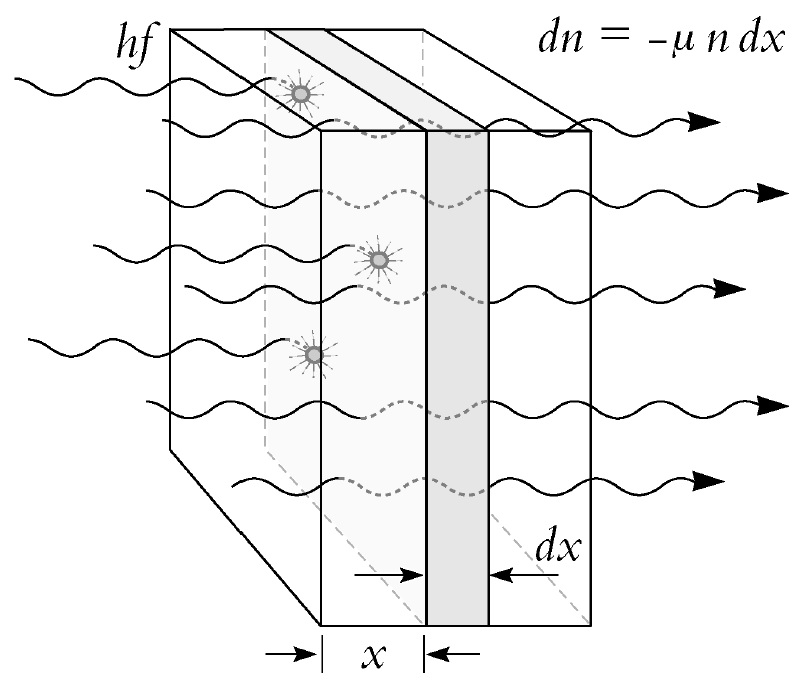
\includegraphics[width=0.45\textwidth]{./fig/l3_attenuation.jpg}
\end{figure}

\begin{equation}
I(x) = I(0) e^{-\mu x}
\end{equation}
 x is the depth into the tissue (units of cm or
m) and $\mu$ is the attenuation coefficient (units
of cm -1 or m -1 ).
{\Large\bfseries\sffamily Most important equation in course.}

 In imaging, primary interest is how much
beam intensity penetrates different parts of
the body to reach the detector.

\begin{example}
Qualitatively describe the different photon –
atom interactions relevant to medical imaging.
– Coherent scattering
– Compton scattering
– Photoelectric effect
– Pair production

 Coherent scattering:
– Photon direction changed slightly by atom.
– Elastic scattering.
– Only significant for low E.

Compton scattering:
– Photon ejects orbiting electron and is scattered in
different direction.
– Inelastic scattering.
– High energy photons only.

 Photoelectric effect:
– Photon of matching energy ejects orbiting
electron.
– Near complete absorption.
– Primarily low energy photons.

 Pair production:
– Photon interacts with nucleus to create positron-
electron pair.
– Complete absorption.
– High energy photons only.
\end{example}


% assignment 1 here
\chapter*{Assignment 1}


\chapter{Image quality [4]}
Key parameters for quantifying image/imaging
quality:
– Spatial resolution
– Contrast
– Signal-to-noise ratio (SNR)
– Fidelity
– Dynamic range
– Field of view (FOV) [视野]
– Temporal resolution [时间分辨率]


Typically impossible to simultaneously achieve
all aspects of image quality.
Realistic images are good in some aspects and
bad in others.

\section{Spatial Resolution}
The spatial resolution
of an imaging system
is how closely two
points can be
separated before
they can no longer be
resolved as distinct
points.

The threshold for resolvability is typically
based on convention.
For light microscopy, the Rayleigh limit.

Different imaging modalities have different
physical principles that limit resolution.

 Spatial resolution mathematically estimated
when designing an imaging system,
 also experimentally checked after
construction and on a regular basis as part of
maintenance.

\subsection{Linear Analysis}
For a \emph{linear, shift-invariant} imaging system, the
image is the convolution [卷积] of the object and the
system's \textbf{point spread function} (PSF).
\begin{equation}
{\rm IMG}(x,y) = {\rm OBJ} (x,y) * {\rm PSF} (x,y)
\end{equation}
 Linear means the image is the summation of
discrete points on the \emph{object} multiplied by the
PSF.
 Shift-invariant means the same PSF can be
applied to every part of the object and.

 1D example of a point object function is 
 \[
 {\rm OBJ}(x)=\delta(x)
 \]

 In a perfect 1D imaging system, the PSF is a
delta function \[{\rm OBJ}(x)=\delta(x)\].

 This would result in OBJ(x) = IMG(x).
 
 \begin{equation}
{\rm IMG}(x_0,y_0) =\iint {\rm OBJ} (x,y)  
{\rm PSF} (x-x_0,y-y_0) \dd{x} \dd{y}
\end{equation}

\begin{example}
\[
{\rm OBJ}(x)=\delta(x+1)+\delta(x-1),{\rm PSF}(x)={\rm sinc}^2\,x.
\]
\[
{\rm IMG}(x)={\rm sinc}^2\,(x+1) + {\rm sinc}^2\,(x-1)
\]
\end{example}

\subsection{Measurement}
Resolution can be measured with an object
containing holes/slits of decreasing size.
• Find the smallest resolvable hole/slit.

Note that improvements in resolution often
come at the expense of SNR.

\section{Contrast}
 Contrast is differences in intensity across the
image representing different structures.

 The physical principles behind contrast differ
between imaging modalities.

• Light: scattering, absorption, fluorescence.
• X-ray: absorption.
• PET: positron emission from contrast agent [造影剂]
• Ultrasound: acoustic impedance.
• MRI: magnetic relaxation times.

\section{SNR} %spatial resolution

SNR can be measured from an image by
computing the mean intensity (signal) and the
standard deviation of intensity (noise).

 Note that spatial resolution and contrast have
rigorous definitions, but the \emph{thresholds of
resolvability} can be varied depending on SNR.

\section{Fidelity}
Image fidelity is how accurately the image
represents the object.

 Fidelity can be affected by imaging artifacts.
 Is there really two heads in the image?

 Artifacts typically represent physical
limitations of the imaging modality [方式].

Common artifacts:
– X-rays: motion, double exposure, foreign objects
-  CT: streaking, shading, rings, distortion
– PET: streak [条纹], attenuation
– Ultrasound: shadowing, acoustic enhancement, …
– MRI: zipper, motion, magic angle, aliasing …

Most artifacts should be avoided by correct
instrument design and use.
• Therefore, the presence of artifacts in an
image likely suggests maintenance or quality
check is required.
• Some artifacts are difficult to avoid and the
clinician must be aware of these to avoid
misinterpreting images.


\section{Dynamic Range}
a finite difference
between the minimum and maximum
intensity pixels in an image.

\section{Field of View}
The field of view (FOV) is the spatial extent of
the object that can be captured in the image.
• Imaging systems with small FOVs can only
image portions of big objects.
• Vice versa, systems with big FOVs can image
the whole of big objects.


\section{Temporal Resolution}
Some imaging modalities offer real-time, or at
least time-resolved, imaging capabilities.

 Examples: x-ray angiography [血管造影], ultrasound.

 Temporal resolution is the shortest change in
structure (eg. heart beat) that can be imaged
by the imaging system.

Trading FOV for spatial and temporal resolution.

Image quality is determined by the physical
limitations of the imaging modality and the
skill of the users.
• Therefore, image quality must be checked on
a regular basis as part of quality assurance.
• Users must also be aware of the limitations of
different imaging modalities.
• Different aspects of quality can be traded,
depending on needs of the application.




\chapter{``planar'' X-ray imaging [5]}
 In x-ray imaging, 2D images are formed by
differential absorption of x-ray beams across
the body.

 X-ray beams travel from the source to the
body.
• The beams are differentially attenuated by the
body.
• Beams penetrating the body differ in intensity
depending on the path they took through the
body.
• 2D intensity pattern is recorded by the
detector.
\[
I(x)=I(0)e^{-\mu x}
\]
This forms Contrast!

Realistic x-ray imaging much more
complicated.
– Scattering
– Noise
– Artifacts
– Motion
– Broad x-ray spectrum
– Mass density or mass attenuation coefficient
differences?
– Detector response

\section{•}

\section{Contrast – Dose Trade-off}
Using harder x-rays (higher energy) that easily
penetrate the body reduces the dose to the
patient as most of the intensity is transmitted.

However, contrast depends on different
structures differentially absorbing x-rays.
Employing x-rays that are readily transmitted [higher energy]
reduces contrast.

Important to optimize contrast vs. dose. 
\[
{\rm \frac{Contract}{Dose}}
\]

Optimal setting can also vary with patient and
different optimization equations can be used.
 An ideal x-ray spectrum for contrast vs. dose
would concentrate photons at one energy.
But Not practical .

\section{Adjusting X-ray Spectrum}
 The x-ray spectrum emitted by the x-ray tube
can be adjusted depending on clinical need.
• Soft x-rays (low energy) can be favored for
improved contrast.
• Hard x-rays (high energy) can be favored for
better penetration.

Heavy metals such as molybdenum (Mo)
absorb x-ray photons of different energies
differently, enabling spectrum shaping.


X-ray spectrum depends on anode-filter pair.

The x-ray spectrum can be shifted up or down
(higher or lower intensity) by changing the x-
ray tube voltage.
\section{Detector}
 A x-ray detector consists of multiple
components.
– Anti-scatter grid for rejecting scattered x-ray
photons.
– X-ray sensitive receptor for converting photons
into light (analog display) or electrical signals
(digital display).
– Film or screen for analog display or computer for
digital display.

Trade-off is less photons reaching detector,
possibly lowering SNR.

 Optimizing scatter rejection to improve
contrast with sufficient SNR requires a
detailed understanding of the impact of
scatter on contrast.

 The rest are either transmitted or scattered
into the detector. The challenge is to distinguish these two.

 An important parameter in x-ray imaging is
the ratio of primary (unscattered) to scattered
photons that reach the detector.
\[
S = \frac{E_{scatter}}{E_{primary}}+1
\]  
The main effect of \textbf{scattering on image quality
is reducing contrast}.

 Contrast increases with grid ratio and
decreases with scatter factor.

Besides a grid, there are other means to
reduce the impact of scatter on contrast.
\begin{itemize}
\item Employ narrow (collimated) beam. [Collimation reduces FOV.]
\item  Have an air gap between patient and detector. [ Air gap makes the instrument larger.]
\end{itemize}

\section{Digital Display}
 A digital x-ray detector consists of a x-ray
sensitive receptor and an A/D converter.

One commonly used receptor is the
stimulable phosphor [激发荧光体] receptor.

A dose proportional amount of energy is
stored by trapping of free electrons and holes.
• Stored energy can be released by scanning
phosphor with laser (stimulated emission).
• The intensity of the emission is measured by a
photomultiplier tube (PMT) and send to the
A/D.

\subsection{SNR}
 In general, the longer the receptor is exposed
to x-rays, the higher the SNR.

 Digital images can be post-processed to
improve image quality and usefulness.

\section{Artifacts [6]}
{\sf Start of Lecture 6}

An artifact [失真] is any image feature that does not
represent an actual structure in the object.

Common x-ray artifacts related to:
\begin{itemize}
\item Image storage and pre-exposure handling

The detector, both screen/film based (analog)
and computer based (digital), is particularly
sensitive to mishandling [处理不当].
• These should be eliminated as part of regular
quality control.

 Film should not be directly contacted with the
fingers, else fingerprints may be added. ...

Both analog films and digital discs/memory
can be affected by accidental exposure [数字暗盒意外曝光].


\item Patient positioning

 the patient
is placed too close or
far from the film.

Sometimes the patient
is initially correctly
positioned but he/she
rotates prior to x-ray
exposure. Leads to distortions.

The x-ray tube (source) and the detector grid
can be misaligned.

\item Exposure

errors
can still occur during the x-ray exposure [X射线]
process.

 Two images may accidentally be recorded on
the same file/disk (double exposure).


\item Processing and reading

The film may not be adequately mixed with
the developer [显影].

For digital detectors, dirty light guides may
obstruct light going from the x-ray receptor to
the photomultiplier tube.


\item Computer workstation

 Errors may also occur at the computer
terminal where images are stored and
displayed.
– Faulty data transfer
– Clipping
– Planking
– Uberschwinger


\end{itemize}



\chapter{Computed Tomography (CT) [7]}
{\sf Start of Lecture 7}


\section{Data }
\begin{enumerate}
\item X-ray beam passes through body, is differentially absorbed in body, and reaches array of detectors (just like planar imaging).
\item The x-ray tube and detector array are rotated around the body and another planar image acquired from different direction.
\item Rotation + acquisition repeated to obtain multiple views (typically > 100).
\item
\end{enumerate}

\section{Reconstruction}
An important concept is how to transform the hundreds to thousands of planar x-ray images into a tomogram (3D image of attenuation).
This mathematical procedure is known as reconstruction and is done by a computer.
Depending on the number of views, the size of each view, and the processing speed of the computer, reconstruction can take seconds to hours.

For an inhomogeneous medium where attenuation varies with depth,
\begin{equation}
I(L)=I_0 e^{-\int \mu(x)\dd{x}}
\end{equation}
Note that in CT, the objective is to measure μ(x) given $I_0$ and I(L).


First define the
absorption (M) of a x-
ray beam travelling
along the line L due to
tissue.
\begin{align*}
x = & r \cos{\theta} - s \sin\theta  \\
y = & r \sin\theta  +  s\cos\theta
\end{align*}
\begin{equation}
M (r,\theta) = \int \mu(r\cos\theta-s \sin\theta,r\sin\theta+s\cos\theta)\,d s
 \iint \mu(x,y) \delta (x\cos\theta+y\sin\theta-r)\,dx\,dy
\end{equation}
Here $r$, $\theta$ is known.

Radon transform 

\subsection{ High pass filtration
followed by back
projection (filtered back
projection)}


Let ${\cal R} [\mu(x,y) ] = M(r,\theta) $ be the Radon transform
of $\mu$. $\mu(x,y) \to M(r,\theta)$

The filtration step involves taking the 1D
Fourier transform of ${\cal R} [\mu]$ about the direction
r ${\cal F}_r$, multiplying by a ramp filter $|\omega|$, than taking
the 2D inverse Fourier transform ${\cal F}^{-1}$.
The last step is to take the back projection of
the filtered Radon transform to obtain $\mu$.
\[
\mu = \frac{1}{2}{\cal B} \left[
{\cal F}^{-1}
\Big[|\omega| {\cal F}_r \big[ {\cal R} [\mu] \big]   \Big]  
\right]
\]

For analytical questions, such as those in this
course, it may be preferable to use the
following integral to compute the filtered back
projection rather than perform a series of
Fourier transforms.
\[
equation goes here
\]

A key of filtered back projection is the central
slice theorem, which states that
\begin{equation}
{\cal F}[\mu](\omega\cos\theta,\omega\sin\theta)
= {\cal F}_r [ {\cal R }[\mu] ] (\omega,\theta)
\end{equation}

\subsection{accuracy}
The accuracy of the reconstruction depends in
part on how completely the Radon transform
is sampled.
\begin{itemize}
\item More $r$ and $\theta$'s, more accurate.
\item Also, highly asymmetric sampling or having
unsampled regions can lead to additional
reconstruction artifacts.
\item In this course we will focus on the continuous
approximation for simplicity.
\end{itemize}


\section{Fourier Transform}
For imaging applications, the Fourier
transform decomposes a spatially defined
function into its spatial frequency
components.
\[ f(x) \overset{FT}{\longrightarrow} F(\omega)\]

The 1D Fourier transform is:
• The inverse transform is:
\begin{equation}
F(\omega) = \int_{-\infty}^{\infty} f(x) e^{-2\pi i \omega x} \dd{x}.
\end{equation}

\begin{equation}
f(x) = \int_{-\infty}^{\infty} F(\omega) e^{2\pi i \omega x} \dd{\omega}.
\end{equation}

• x has spatial dimensions (eg. meters) and ω
has spatial frequency dimensions (eg. m -1 ).


\begin{example}
A simple point object $\mu{x,y}=\delta(x,y)$\footnote{This is a 2D delta, $\mu$ goes like $1/r^2$}.
Compute the Radon transform to obtain what
the CT scanner would measure.
\begin{align*}
M(r,\theta)
=  &
\iint \mu(x,y) \delta (x\cos\theta+y\sin\theta-r)\,dx\,dy  \\
=  &
\iint \delta(x,y) \delta (x\cos\theta+y\sin\theta-r)\,dx\,dy  \\
=  &
  \delta(-r)=\delta(r)
\end{align*}

 Only the source-detector pair corresponding
to the x-ray beam passing through the middle
of the object (r = 0) detects absorption.

Note that we have not accounted for the fan
beam geometry typically employed by CT
scanners to best use a x-ray tube.
\end{example}

\begin{example}
 The object: $\mu(x,y)$.
\begin{center}

\includegraphics[width=0.2\textwidth]{./fig/l7_ct_obj.jpg}
\end{center}
 

 The Radon transform: $R[\mu](r,\theta)$.
 \begin{center}
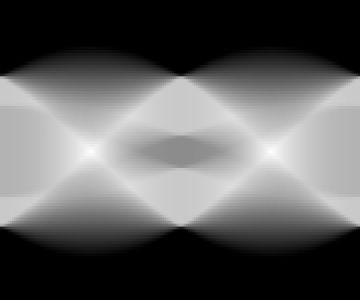
\includegraphics[width=0.2\textwidth]{./fig/l7_ct_rt.jpg}
\end{center}
 
 The unfiltered back projection: $B[R[\mu]](x,y)$.
 
 Filtered back projections with various views:
\end{example}




\section{Hardware [8]}
{\sf Start of Lecture 8}

 A CT scanner is a planar x-ray instrument with
additional hardware to rotate the source and
detector, translate the patient, and
reconstruct the images.


\subsection{Gantry}
 The gantry is the rotating core of the scanner.
  The gantry consists of:
– X-ray tube

discussed in lecture 1

– Detector(s)

Detectors in CT are digital.
• Scintillation detectors often employed.
Scintillation crystal emits light when irradiated
by x-rays.
Light is converted into electrical signal and
digitally stored for processing.

– Collimators/Filters

 Collimators  reduce unnecessary patient
dose and improve image quality.
• There are two types of collimators, pre and
post patient collimators.

Very similar to grids used in planar imaging.
• Collimators are also used in planar imaging to
more precisely define the x-ray beam and
reject scattered photons.

 The x-ray flux is homogenous in the umbra as
the beam is not blocked by the pre-patient
collimator.
• The penumbra is inhomogeneous as the beam
is partially blocked.
• For single slice CT, both regions are used for
imaging, so the blockage in the penumbra
must be carefully measured.
• For multi slice CT, only the umbra is used.

 Filters attenuate the low energy (soft) x-rays
to reduce the unnecessary dose.
• Filters are made of medium Z materials that
preferentially absorb soft x-rays. 
 Recall that soft x-rays cannot penetrate the
patient and thus, are not useful for imaging.

There are two types of commonly used filters:
flat and bow-ti [领结]e.


– Slip rings [集电环]

 Slip rings allow smooth, continuous rotation of
the gantry while delivering electrical power.


– Motors

 The motor of a CT scanner must turn the
heavy gantry at high speeds and with high
accuracy and precision.

 In CT, the scanner is typically rotated by a
\textbf{direct drive motor} capable of providing
around 1000 views per revolution.

– Microprocessors

control the
– rotation of the gantry,
– translation of the patient bed,
– tilting of the gantry,
– turning on and off x-ray tube,
– and acquisition by the detector.


– Positioning lasers

This further refines the positioning of the
patient relative to the gantry and the room.

\subsection{Control Console}
A CT scanner is considerably more complex
than a planar x-ray system and requires a
dedicated operating console.

The console serves two primary purposes:
– input the scan parameters
– and display the reconstructed images.

\subsection{Computer}

 CT scanners have high performance
computers for image reconstruction.
• Image reconstruction is a computationally
expensive procedures that requires high
processor speeds and large memory.

\section{Software}

 The filtered back projection is the primary
reconstruction algorithm and is considered an
analytical reconstruction method.
• The key to fast reconstruction using filtered
back projection is the fast fourier transform.
• Recall from the previous lecture that FFT is
${\cal O}(n \log n)$ implementation of the discrete
fourier transform.

Wolfram MathWorld
(\url{http://mathworld.wolfram.com/FastFourierTransf
orm.html})

The second common type of reconstruction
method is iterative reconstruction.
• Analytical reconstruction is a one step
algorithm while iterative reconstruction
performs multiple steps.
• The image after each step is used to define
the reconstruction of the next step.

 The raw CT images must be converted into the
format desired by the radiologist.

Rendering includes:
– Interpolating images into a new space depending
on the orientation and magnification at which the
radiologist wants to view the image.
– Adjusting contrast and brightness.
– Adding false color.

\section{Artifacts}
 In lecture 6 we discussed commonly seen
artifacts in planar x-ray imaging.
• There are also artifacts specific to or especially
problematic in CT.
• Some common ones are:

– Motion

 Due to the longer duration of CT scans,
compared with planar x-rays, there is greater
susceptibility to motion artifacts.

– Partial volume averaging [部分容积]

an image
voxel [三维像素] (3D version of a pixel) contains two
distinct image features (eg. bone vs. muscle).

– Streaks [条纹]

 Streak artifacts occur around materials that
block x-rays, such as bones.


– Low SNR

when image slices are set to
be too thin and thus, an insufficient number
of photons reach the detector.



\chapter{Magnetic Resonance Imaging (MRI) [9]}
{\sf Start of Lecture 9}

 A wide range of intrinsic contrasts are
available, for example:
– muscle vs. fat vs. ligaments
– blood flow and that of other fluids
– water diffusion
• Contrast agents [造影剂] can also be used.


\section{History}
MRI extends the principles of the \textbf{nuclear
magnetic resonance} (NMR) phenomenon to
3D imaging.
• NMR is still an important chemistry research
technique today.
• MRI was originally called nuclear magnetic
resonance imaging, but “nuclear” was
dropped to avoid association with nuclear
weapons and nuclear waste.

\section{Basic Physics}
 All atomic nuclei (eg. H) have a physical
property called spin.
• The \emph{spin of a nucleus} is a physical property
just like atomic number, atomic mass, etc.
• Isotopes with an odd number of protons and
neutrons have non-zero spin. Examples include ${^1 H}$ and $^{13} C$.
• Electrons also have spin and can be measured
with electron paramagnetic resonance (EPR).

 In NMR and MRI, an \emph{external electromagnetic
field, typically at radiofrequency} (depends on
field strength), tips $\vb{M}$ away from $\vb{B}$.
• In MRI, M is usually tipped 90⁰ or 180⁰ from B.

 MRI involves tipping spins and measuring the
time to relax back to the pre-excitation state.
• This is known as relaxation time.
• Different tissues have different relaxation
times.
• So far this discussion applies to 1D NMR and
3D MRI.

 There is a one to one relationship between
the magnetic field strength and the frequency
of electromagnetic radiation that can tip M.

• Similarly, the frequency of electromagnetic
radiation released by the spins upon
relaxation also has the same one to one
relationship with the field strength.


\subsection{3D Imaging}
 The key to 3D imaging is to have slightly
different magnetic field strengths (several mT)
across the body.
• That way, a narrowband electromagnetic
pulse will only excite spins in a portion of the
body.
• Further, when those spins relax, they will emit
electromagnetic radiation of different
frequencies.


 A MRI scan consists of repeated RF excitations,
each time with different combination of
gradients.

 A 2D Fourier transform is used to reconstruct
the image from recorded FIDs (signals).

\section{Hardware}
MRI systems consist of several key
components:
\begin{itemize}
\item superconducting coil for high field strength
magnetic field (> 1 T)
\begin{equation}
B = \mu_0 n I
\end{equation}

 For B to be large (several T), I must be large.
• For I = V/R (Ohm’s Law) to be large, V must be
large and R must be small.
• Therefore, the magnet is a high voltage, high
power device cooled by liquid nitrogen and
helium to minimize R

\item gradient coils for magnetic field gradients

 Gradient coils generate small magnetic fields
along multiple directions to create controlled
inhomogeneities in the overall field. Typically a set of 3 coils.

A “gradient” can be introduced into the
magnetic field along any of the 3 directions.


\item transmit and receive RF coils

 Radiofrequency coils are important for
transmitting and receiving RF signals to and
from the body.

Coils must be well tuned to have a clear
resonance frequency as all RF signals
employed by the MRI scanner will be within a
narrow bandwidth.
\[
\omega_0=\frac{1}{\sqrt{LC}}
\]
\item cooling system
\item patient accessories

 A number of patient accessories are used
during MRI scans.
• Accessories for monitoring vital signs:
– heart rate
– respiration rate
– body temperature
– blood oxygenation
– electrocardiogram
• Must be MRI compatible!

\item computer
\end{itemize}

\section{Image reconstruction}
[skip, no details]

 There are different ways to sample k-space.
 These ways are pulse sequences.
 \begin{itemize}
\item Some sequences are slower but provide
higher quality images (typically used in
medicine).
– Rapid acquisition with refocused echoes.
\item Some sequences are faster but sacrifice image
quality (typically used in research).
– Echo planar imaging
 \end{itemize}
 


 k-space can be converted to image space by a
\emph{2D Fourier Transform} (see lecture 7).
• A Fourier Transform can be computed using
the Fast Fourier Transform (FFT) algorithm,
making MRI image reconstruction very fast.
• Reconstruction of large images can be done in
seconds using standard computers.
• \emph{Very different from CT reconstruction.}


\section{Safety}
Therefore, nothing with iron can be placed
near a MRI scanner.
 MRI scanners are held in dedicated rooms
with the 5 gauss line clearly labelled.

 All accessories must be MRI compatible.
• This means no iron.
• Also, electronic circuits made with copper
wires do not work in MRI scanners because of
the many RF signals.
• The RF signals will induce unwanted currents
in the wires, interfering with device operation.


\chapter{Nuclear Medicine Imaging [10]}
 In many major hospitals, medical imaging is
divided between two closely related
departments.
• Primary department is Radiology.

 The other department is Nuclear Medicine
(NM). [核医学]

Nuclear medicine imaging differs from other
methods of imaging, particularly x-rays, in that
the radioactive source of contrast is injected
into the body.
 Further, NM imaging primarily images body
function while other methods primarily image
body structure.

The radioactive isotopes are typically bonded
with a ligand [配体] specific to certain tissue types
(eg. cancer). This allows the resulting
radiopharmaceutical [放射性药物] to accumulate in the
region of interest.

\section{Uptake ((one data point))}

Uptake is the fraction of an
administered [施用(药物)] radionuclide
that accumulates in the
organ of interest at
selected times following
ingestion.

A similar measurement is taken from a
phantom [与人体组织等效的“模体”] designed to mimic the organ.

 Consider an $^{131}I$ source accumulating in the
thyroid:
– attenuation
– $1/r^2$
– scattering

So, $I(r)\sim e^{-\mu r} \frac{1}{r^2}$

The effects of scattering, attenuation, and etc.
can in principle be modeled from first
principles.
 However, accounting for these losses is
typically done through a combination of
Monte-Carlo simulations and phantom
measurements.

Radiopharmaceuticals typically contain a
metabolically [代谢] relevant ligand (eg. glucose [葡萄糖]).

functional imaging methods

\subsection{Scintigraphy}
Scintigraphy [显像] is the basic form of 2D nuclear
medicine imaging and is one of the most
frequently used forms of NM imaging.
Role is similar to that of planar x-ray imaging.

Radiation, typically gamma rays, is emitted
from the organ and detected by an external
detector called a scintillator [闪烁体] (aka. gamma
camera).
 The gamma camera is a 2D camera that
converts gamma rays into visible light that is
recorded by photodetectors.

However, the measured signals are not usually
calibrated with phantoms, meaning they are
more qualitative.

Scintigraphy is performed in multiple organs:
\begin{itemize}
\item  bile ducts [胆管] (gall bladder [胆囊])
\item lung

Lung scintigraphy used to diagnose pulmonary
emboli [肺栓塞] (blockage of artery in lung).

${\rm ^{99m} Tc}$ [m for metastable 锝-99m] is the radionuclide used, typically in
aerosol [气雾剂] form and inhaled into the lungs or via
iv injection.
${\rm ^{99m} Tc}$ has a half-life of 6 hours and primarily
emits gamma rays at 140 keV. The \emph{most frequently used radionuclide in
nuclear medicine imaging}.
Produced via portable generators from 99 Mo
(half-life of 66 hours).

Typically a 100 MBq source of 99m Tc is used.
• The distribution of the radionuclide is related
to the air flow in the lungs (inhalation [吸入]) or the
blood perfusion (iv injection).
• Images are acquired shortly after the
radionuclide is introduced.

\item

Bone scintigraphy used for detection of bone
cancers and injuries.

99m Tc-Methyl diphosphonate[二磷酸甲酯]

\item thyroid [甲状腺] and parathyroid [甲状旁腺]

Scintigraphy is used in the detection and
diagnoses of a range of thyroid conditions,
including cancer and hyperthyroidism.

Iodine naturally builds up in the thyroid,
making the radioactive isotopes well suited to
thyroid imaging.

\item kidney 

Scintigraphy is used to examine kidney
clearance [肾清除率], the rate at which waste substances
are removed from the kidneys.
\end{itemize}


Cardiac [心脏的] scintigraphy is used in a number of
medical applications.
– first pass [首次通过] studies
• myocardial function
– blood pool scanning 37
• blood volume

Blood pool scanning involves injection of the
radionuclide followed by gated measurement
of dynamic blood volume changes.
• Able to measure blood volume at different
stages of the heart beat.


\subsection{SPECT}
Single-photon emission
computed tomography
(SPECT) is the 3D version of
2D scintigraphy.
The relationship between
2D scintigraphy and SPECT
is very similar to the
relationship between
planar x-ray imaging and
computed tomography (CT).

Note that radiation is always being emitted
from the radionuclides in all directions.
• The camera(s) are rotated around the body to
record radiation emission from different
directions.
• This differs from CT where the radiation is
switched on and off.



SPECT is often used to image the heart and
brain:
– myocardial perfusion [心肌灌注] (blood flow in the heart
muscle)
– functional brain imaging (image brain activity)


 SPECT is routinely acquired simultaneously
with CT using dual modality systems.
• This enables matched structural and
functional imaging of the subject.

\subsection{PET}
Positron emission tomography (PET) is
arguably the most advanced form of 3D NM
imaging and one of the most advanced forms
of medical imaging.

The radionuclides used in PET are different
from those used in SPECT because PET
detectors are not conventional gamma
cameras.
 
  One common PET radiopharmaceutical is 18 F-
FDG (fluorodeoxyglucose).

After annihilation, two 511 keV photons are
created travelling in opposite directions.
• The photons are collected by scintillators
(gamma -> light detectors) outside the body.

PET detectors are designed to detect near
simultaneous arrival of two photons (within
several nanoseconds) while ignoring individual
photon arrivals.  This improves noise rejection as two noise
photons are unlikely to arrive simultaneously.

Unlike SPECT detectors, PET detectors are
coincidence detectors, not 2D cameras.

Each pair of photons can be used
to trace the location of the
annihilation event to a line
connecting the detector elements.
• \textbf{However, the temporal resolution
of the detectors typically cannot
pinpoint the site of annihilation.}


\paragraph{TOF} Some cutting edge PET scanners have
detectors with adequate temporal resolution
to localize the annihilation event to several
centimeters by using time-of-flight (TOF).

 Each event will emit two photons, but in
random (but opposite) directions.
• Therefore, the same tissue site will send
photons to all detectors.
 Similarly, each detector will receive photons
from all tissue sites.
• TOF + detector counts used to reconstruct a
map of radionuclide distribution.

Many radionuclides used in PET have short
half lives.
• Therefore, very important for a hospital to
have a local source of radionuclides.
• Cyclotron or portable generator.
• For radionuclides with half-lives of just several
minutes, the cyclotron/generator may need to
be right next to the PET scanner.

Cancerous tissues divide
rapidly compared with
normal tissues and thus, will
be more metabolically active, glucose analog
that is uptaken by tissues,
with the uptake proportional
to the metabolic rate. \footnote{Spatial resolution of PET is low.}

Therefore, the biological half-life of FDG is
very similar to the radioactive half-life.

A variety of radiopharmaceuticals [放射性药物] can be
employed to selectively image different
neuroreceptors in the brain.

 Like SPECT, PET is also regularly combined
with CT and MRI in dual modality systems.


 At present, NM is limited by cost and
operational complexity.

\section{Gamma Detector [11]}

Nuclear medicine imaging typically requires
sensitive detection of gamma rays emitted
from the body at low intensities.
\subsection{Geiger-M\"{u}ller counter}


Townsend avalanche (雪崩) phenomenon

One gamma-ray would produce millions of electrons.

Geiger-M\"{u}ller contour is for low intensity. Since the time for
the avalanche is around several microsecond.

\subsection{Scintillation detectors}
Scintillation (闪烁体) detectors use

\begin{itemize}
\item high $Z$ (atomic number) to favor 
\textbf{photo-electric absorption} over Compton scattering, [inner electron
knocked out]
\item high {\sf gamma ray to photon ratio};
\item low absorption at wavelength of generated photon;
\item Index of refraction should be close to 1.5, that of glass, to facilitate coupling with the \textbf{photomultiplier tube} (PMT 光电倍增管). To let the light photon goes effectively from 
\end{itemize}


Dynodes 倍增极

\subsection{Gamma camera}
Gamma cameras are basically an array of scintillation detectors.

scintillation effect different region --- and spatial reso -- and close camera.


\subsection{PET Detector}

\paragraph{TOF}



\section{radiopharmaceutical handling}
Radiopharmaceuticals are usually injected into
the patient intravenously [静脉滴注].
• The syringe [注射器] must shield the radiation from
hospital staff.
• At the same time, the syringe must be able to
get the radiopharmaceutical into the patient.

One example is syringes for iv [Intravenous] injections.

\section{image registration}
Modern NM imaging is often combined with
anatomical imaging by CT or MRI.
• This requires that the metabolic images be
registered with the anatomical images.
• There are algorithms for image registration [图像配准]
suited for different acquisition methods.





\chapter{Ultrasound Imaging [12]}

\section{Physics}
Ultrasound physics are very different from x-
ray, gamma ray, and MRI physics.

 In ultrasound, \emph{high frequency} acoustic
pressure waves (MHz range) are sent into the
body by a transducer.
 The sound waves are reflected by acoustic
interfaces within the body.

The reflected waves
are recorded by the
transducer.
• Both the amplitude
and return time of
the waves are
recorded.
• These are used to
reconstruct an
image.

 If there are moving objects inside the body
(eg. blood flow), the frequency of the
returning sound waves are different from that
of the original wave. This is known as the \textbf{Doppler Effect}.

The Doppler Effect is used in Doppler
ultrasound to measure the direction and
speed of blood flow.
• The direction of flow is usually color coded.

\section{hardware and
software}
In this lecture, we will focus on hardware and
software in ultrasound imaging.

\begin{itemize}
\item transducer

It is responsible for sending sound pressure
waves into the body and converting the
returning sound waves into electrical signals.

Transducers are based on piezoelectric
materials.
 Piezoelectrics expand or contract in the
presence of an electric field.
 Conversely, expansion or contraction of a
piezoelectric will generate an electric field.

 If the piezoelectric is connected to an
electrical circuit with a MHz frequency AC
source, the piezoelectric will vibrate at the
same MHz frequency.
• This is the basis of ultrasound transmission.



\item image reconstruction

\url{https://en.wikipedia.org/wiki/A-scan_ultrasound_biometry}

\item 3D/4D ultrasound

Ultrasound is primarily used in B-scan (2D)
mode, where video rate imaging with large
field of view is readily achieved.
• 3D ultrasound involves performing multiple B-
scans to cover a 3D volume.

 4D ultrasound refers to 3D ultrasound imaging
performed fast enough to achieve video rate.
• 3D/4D ultrasound has gained general
attention by enabling parents to “see” their
child in utero (in the uterus).


\item display / control console

One of the strengths of ultrasound
imaging is the compact size of the
instrumentation.
• This enables small, private clinics
to operate multiple ultrasound
systems.

• The ultrasound system’s console
houses the MHz electronics,
image reconstruction computer,
and display monitor.

Video rate ultrasound imaging requires a
specialized console that allows doctors and
nurses to more easily acquire and interpret
video images.


\end{itemize}


A typical ultrasound unit is able to perform
different forms of ultrasound imaging.
– standard B-scans (structure)
– doppler ultrasound (blood flow)

For doppler imaging, the false color indicating
flow direction and speed needs to be overlaid
onto the structural images.
• Since the structural images are constantly
changing, the doppler information needs to be
updated in real time.

– M-scan (motion)

For M-scans, the line of investigation must be
defined on the structural images.
• Therefore, there are similar requirements to
making measurements or defining a new field
of view.
• Typically, a frame capture needs to be
performed prior to selecting the line.


\end{document}
